\documentclass[thesis.tex]{subfiles}

\begin{document}

\externaldocument[C3-]{build/chapter03}
\externaldocument[C4-]{build/chapter04}

\chapter{Wireless Capsule Endoscopy}  \label{wireless_capsule_endoscopy}
%-----------------------------------------------------------
%general info about WCE, some history etc
The basic technology behind the modern endoscope was developed in the early 1950s by English physicist Harold Hopkins and his student Narinder Kapany which let light travel through flexible pieces of glass, now known as optical fibers \cite{NewMethod54}.

Before the year 2000 the only option you had to visualize the foodpipe, stomach, duodenum, colon and terminal ileum (see Figure \ref{C3-fig:digestive_system} for details) was to use a fiber-optic endoscope, which is a tool with a relatively wide cable that is pushed into the bowel with as much as 50 000 optic fibers (as seen on Figure \ref{fig:fiber-optic-endoscopy}). These cables have to carry fiber optic bundles, water pipes, operations channel and control cables. Although these cables can be quite flexible there is a limit for how far they can advance into the small bowel. This method cause pain and discomfort for the patient, and there was a clinical need for an improved methods.

\begin{figure} % fibre-optic-endoscope
  \begin{center}
    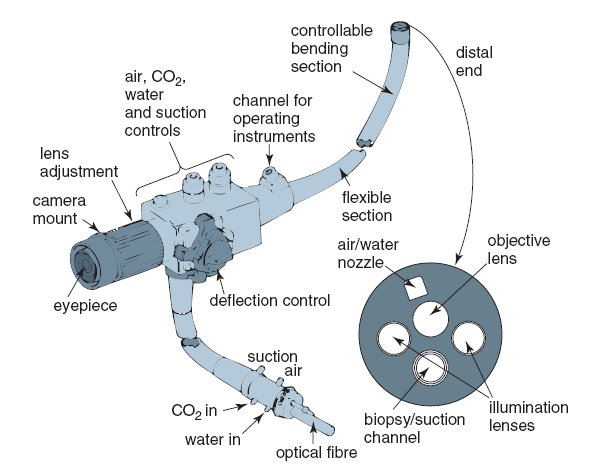
\includegraphics[width=0.7\textwidth]{fiber-optic-endoscope.jpg}
    \caption[Image]{Image of a fibre optic endoscope with explanation of different parts of the tool\footnotemark.}
    \label{fig:fiber-optic-endoscopy}
  \end{center}
\end{figure}

\footnotetext{
\text{Image credit: Jacaranda Physics 1 2nd Edition © John Wiley \& Sons, Inc.}
}



That is why in the year \citeyear{WirelessCapsule00} \citeauthor*{WirelessCapsule00} developed a new type of video-telemetry capsule endoscope that was swallowable \cite{WirelessCapsule00}. It could travel through the entire digestive system because it had no external wires, fiber-optic bundles or cables of any sort. The capsule travels by peristalsis\footnote{Peristalsis is a radially symmetrical contraction and relaxation of muscles that propagates in a wave down a tube, in an anterograde direction.} through the gastrointestinal tract, which takes from 10 to 48 hours, and transmit images on a regular interval to receivers attached around the outside of the patients stomach for as long as the battery allows, usually in the range 6 to 8 hours. Two example images taken by WCE are presented in Figure \ref{fig:pillcam_examples}. By triangulating the signal strength and the location of the receivers taped on the body it is possible to roughly estimate the position of the capsule. This is however not very precise and can not tell us the rotation or direction of the capsule. Regardless, that information will not be available for us in this study as we only have access to the images themselves. Therefore we could implement an algorithm to predict which region of the degistive system the image is taken from (see section \ref{C4-neural_network_models} and \ref{mapping}).

\begin{figure} % fig:pillcam_examples (double figure)
  \centering
  \begin{subfigure}[b]{0.4\linewidth}%
    \centering
    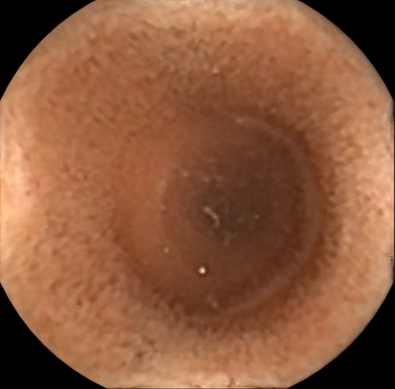
\includegraphics[width=\linewidth]{pillcam_small_intestine}%
    \caption{Small Intestine}%
    \label{fig:pillcam_small_intestine}%
  \end{subfigure}%
  \quad
  \begin{subfigure}[b]{0.4\linewidth}%
    \centering
    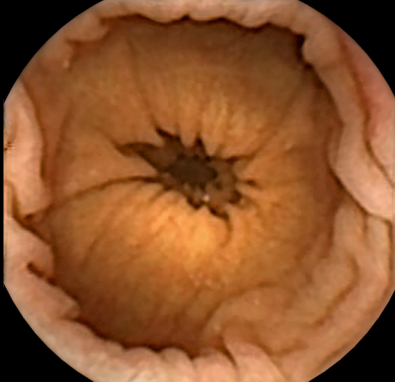
\includegraphics[width=\linewidth]{pillcam_colon}%
    \caption{Colon}%
    \label{fig:pillcam_colon}%
  \end{subfigure}%
  \caption[Images taken with WCE]{Images taken with WCE\footnotemark.}%
  \label{fig:pillcam_examples}%
\end{figure}%

\footnotetext{
\text{CC BY-SA 3.0 / Attribution to Dr.HH.Krause at English Wikipedia;} \newline
\url{https://commons.wikimedia.org/wiki/File:Normales_Colon.PNG} \newline
\url{https://commons.wikimedia.org/wiki/File:Dunndarm.PNG} %Dünndarm
}


\end{document}
